\section{Experiments}
\label{sec:experiments}

The experiments test whether residual-driven repair is useful under deployment gating. We avoid a broad dominance claim and instead ask five questions: when does C5 accept, which components matter, whether the behavior transfers to procedural noisy meshes, whether the accepted spot/PartUV case is stable under held-out light, view, and noise changes, and whether the PartUV repair preserves part-aligned chart structure relative to xatlas.

\subsection{Setup and baselines}
\label{sec:exp_setup}

The main oracle-PBR evaluation uses three assets: spot, bunny, and an Objaverse asset. Each is evaluated with four initial atlases: xatlas, Blender Smart UV, PartUV \cite{wang2025_partuv_part_based_uv}, and a matched oracle atlas. The transfer evaluation uses eight procedural noisy meshes with PartUV initialization. All methods share the same mesh, texture budget, three-split view/light protocol, and PBR baker. Candidate search uses only the proposal split, C5 accepts or rolls back on the gate split, and headline \PSNR{}/\SSIM{}/\LPIPS{} are reported on the test split. Metrics include relit \PSNR, \SSIM, \LPIPS, PBR channel residuals, seam error, mip leakage, distortion tail, utilization, chart count, edited chart count, and C5 verdict.

We deliberately freeze the upstream atlas before repair. This reflects a pipeline where PartUV's semantic, part-aligned charts may be needed for downstream editing, accessory replacement, or rig-aware authoring. xatlas is a strong production-style baseline and often has higher PSNR in our main table, but it globally re-charts the mesh and can lose that part alignment. We quantify this with chart--part purity, using the PartUV leaf-chart partition as the reference part proxy. The reported method therefore asks a narrower question: given the atlas the pipeline has chosen, can local residual-backed edits improve PBR deployment without replacing the atlas family?

PartUV is a real integrated baseline in the final baseline and Main Anchor Evaluation runs. FlexPara \cite{zhao2025_flexpara_flexible_neural_surface}, OT-UVGS \cite{kim2026_ot_uvgs_revisiting_uv}, Flatten Anything, ParaPoint, and a visibility-parameterization control were attempted but not used as full main-table reproductions. Their software or checkpoint blockers are reported in \cref{app:baseline_failure}. This distinction is important: main numerical comparisons are only made against baselines that were actually available under the same evaluation harness.

\subsection{Main results}
\label{sec:main_results}

\begin{table*}[t]
\centering
\scriptsize
\caption{Main Anchor Evaluation results with candidate and deployed outputs separated. Panel (a) reports PSNR before C5 deployment; panel (b) exposes the C5 audit columns used to accept or roll back each candidate.}
\label{tab:main}
\begin{tabular}{@{}llrrrrl@{}}
\toprule
\multicolumn{7}{@{}l}{\textbf{(a) Relit PSNR and deployment}}\\
Asset & Baseline & Init PSNR & Candidate PSNR & Final PSNR & $\Delta$Final & C5 \\
\midrule
bunny & Blender UV & 36.22 & 35.74 & 36.22 & +0.00 & rollback \\
bunny & oracle & n/a & n/a & n/a & -- & rollback \\
bunny & PartUV & 28.30 & 38.53 & 38.53 & \textbf{+10.23} & accept \\
bunny & xatlas & 43.25 & 42.88 & 43.25 & +0.00 & rollback \\
objaverse & Blender UV & 29.81 & 27.80 & 29.81 & +0.00 & rollback \\
objaverse & oracle & n/a & n/a & n/a & -- & rollback \\
objaverse & PartUV & 34.41 & 40.42 & 34.41 & +0.00 & rollback \\
objaverse & xatlas & 45.50 & 45.68 & 45.50 & +0.00 & rollback \\
spot & Blender UV & 43.04 & 40.10 & 43.04 & +0.00 & rollback \\
spot & oracle & n/a & n/a & n/a & -- & rollback \\
spot & PartUV & 30.32 & 44.99 & 44.99 & \textbf{+14.67} & accept \\
spot & xatlas & 49.77 & 47.83 & 49.77 & +0.00 & rollback \\
\bottomrule
\end{tabular}

\vspace{0.5em}
\begin{tabular}{@{}llrrrrl@{}}
\toprule
\multicolumn{7}{@{}l}{\textbf{(b) C5 audit for the candidate atlas}}\\
Asset & Baseline & $\Delta$Seam & $\Delta Q95$ & $\Delta$Util & $\Delta$Charts & C5 verdict \\
\midrule
bunny & Blender UV & -100\% & +0.00 & -0.17 & -1 & rollback \\
bunny & oracle & +0\% & +23.36 & -0.19 & +0 & rollback \\
bunny & PartUV & -82\% & +2.55 & -0.37 & +0 & accept \\
bunny & xatlas & +18\% & +13.68 & -0.26 & +0 & rollback \\
objaverse & Blender UV & -34\% & +0.55 & -0.66 & +0 & rollback \\
objaverse & oracle & +0\% & +1.05 & -0.34 & +0 & rollback \\
objaverse & PartUV & +42\% & +6.69 & -0.25 & +0 & rollback \\
objaverse & xatlas & -4\% & +0.70 & -0.35 & +0 & rollback \\
spot & Blender UV & +44\% & +2.46 & -0.17 & +0 & rollback \\
spot & oracle & +0\% & +37.22 & -0.10 & +0 & rollback \\
spot & PartUV & -90\% & -0.90 & -0.15 & +0 & accept \\
spot & xatlas & -15\% & +30.61 & -0.37 & +0 & rollback \\
\bottomrule
\end{tabular}
\end{table*}


\begin{figure}[t]
  \centering
  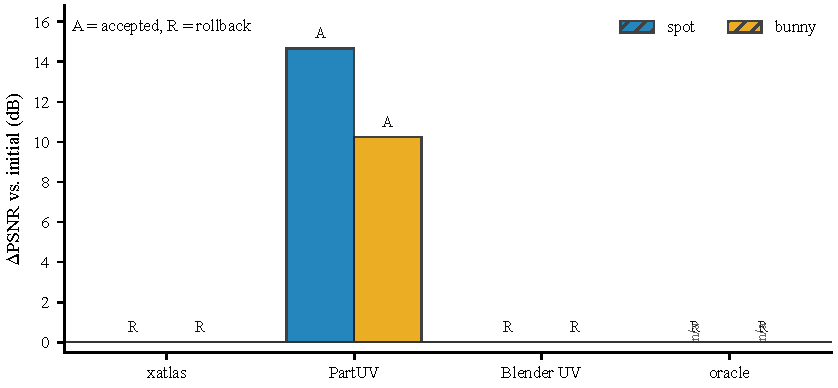
\includegraphics[width=0.95\linewidth]{figures/main/fig3_comparison.pdf}
  \caption{Main Anchor Evaluation comparison on spot and bunny. Positive bars indicate deployed PSNR gain over the initial atlas; labels show whether the C5 gate accepted the repair or rolled back to the baseline.}
  \label{fig:main_comparison}
\end{figure}

\Cref{tab:main,fig:main_comparison} show the central result. The method accepts only two of 12 main cases: spot/PartUV improves from 30.32 dB to 44.99 dB, and bunny/PartUV improves from 28.30 dB to 38.53 dB. All xatlas, Blender UV, Objaverse, and oracle rows roll back to the baseline. This is the intended C5 behavior. xatlas is already strong on these assets, the oracle rows have no meaningful room for improvement, and the Objaverse case has too few editable charts for the local action space to have leverage.

\begin{table}[t]
\centering
\scriptsize
\caption{A1 structural rerun: proposal/gate/test 3-split with multi-seed (n=3). Headline PSNR is on the held-out test split only; candidate search and C5 use disjoint splits. PSNR is mean$\pm$std over split seeds.}
\label{tab:a1_split}
\begin{tabular}{@{}llrrrrl@{}}
\toprule
Asset & Baseline & n & Init PSNR & Final PSNR & $\Delta$Final & Accept \\
\midrule
spot & xatlas & 3 & 48.71$\pm$0.88 & 48.71$\pm$0.88 & 0.00$\pm$0.00 & 0/3 \\
spot & PartUV & 3 & 31.20$\pm$0.40 & 43.78$\pm$1.23 & \textbf{12.58$\pm$0.83} & 3/3 \\
bunny & PartUV & 3 & 28.21$\pm$0.08 & 40.05$\pm$0.81 & \textbf{11.84$\pm$0.89} & 3/3 \\
objaverse & xatlas & 3 & 45.01$\pm$0.93 & 45.01$\pm$0.93 & 0.00$\pm$0.00 & 0/3 \\
\bottomrule
\end{tabular}
\end{table}

\Cref{tab:a1_split} reports the A1 structural rerun: views and lights are split into disjoint proposal, gate, and test sets (\cref{sec:exp_setup}), so candidate search and C5 acceptance never touch the test split that we report PSNR on. Two accepted PartUV cases (spot, bunny) and two rollback controls (spot/xatlas, Objaverse/xatlas) are repeated under three split seeds; the \texttt{ts\_animal} real-mesh case stays single-seed in \cref{tab:real_mesh} (it is sourced through the transfer wrapper and is not retargetable to the B3 multi-seed harness in this submission). The accepted gains hold under the test split with comparable magnitude (spot/PartUV $+12.58 \pm 0.83$ dB, bunny/PartUV $+11.84 \pm 0.89$ dB) and the rollback controls remain at exactly $\Delta=0.00 \pm 0.00$ dB across all three seeds, so the headline gains are not an artifact of evaluating on the same held-out signal used for residual attribution.

\begin{figure*}[t]
  \centering
  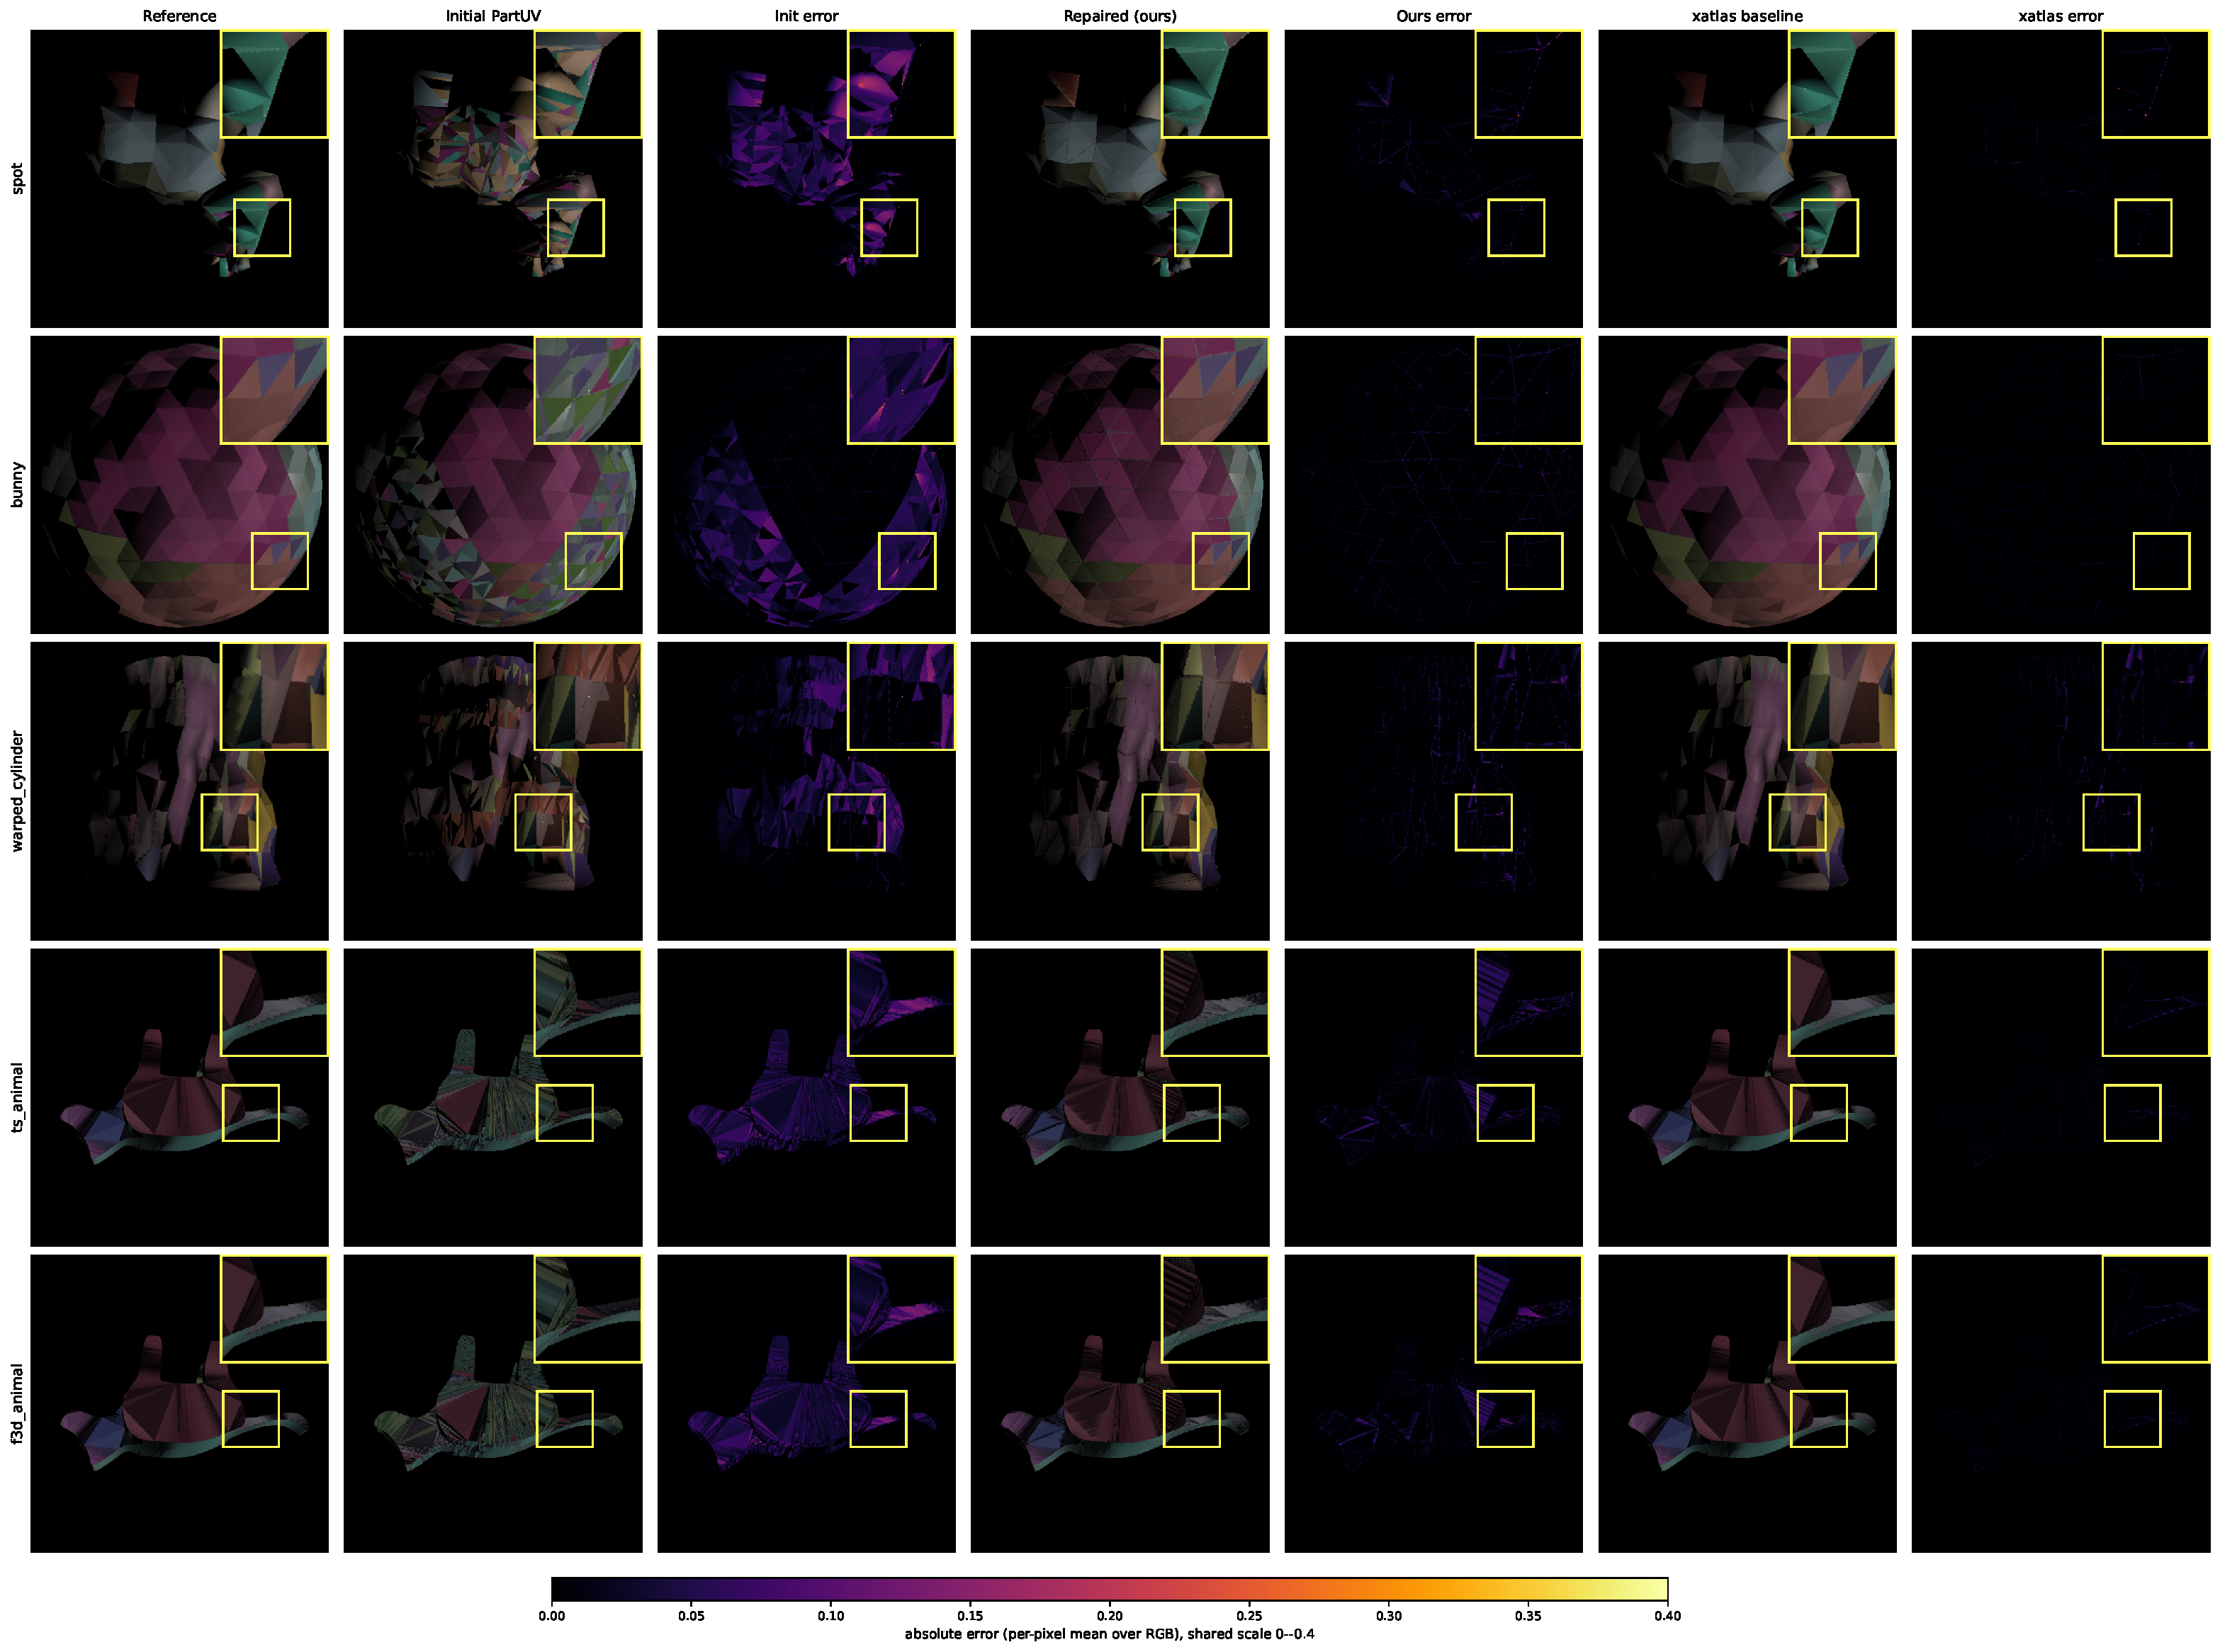
\includegraphics[width=0.78\linewidth]{figures/visual_evidence/fig7_visual_comparison.pdf}
  \caption{Held-out relit before/after for all five accepted cases. Columns: oracle reference; initial PartUV render; init absolute error vs reference; our repaired render; our error; xatlas-baseline render; xatlas error. All rows share the same inferno colorbar (per-pixel mean absolute error over RGB, 0--0.4) at the bottom. The yellow boxes mark the highest-error region in each row's initial PartUV image, with a zoomed inset (top-right of each panel) showing the same region across the seven columns so seam/mip detail is readable at paper scale. Our repair closes most of the gap from initial PartUV to oracle reference; xatlas is sometimes competitive in absolute error but globally re-charts the mesh and breaks the upstream PartUV chart organization (\cref{sec:exp_setup,tab:purity}). The figure therefore supports both the repair improvement and the partition-preservation trade-off.}
  \label{fig:visual_comparison}
\end{figure*}

\Cref{fig:visual_comparison} shows the held-out relit appearance for all five accepted cases (controlled spot/PartUV and bunny/PartUV, procedural warped\_cylinder/PartUV, and real \texttt{ts\_animal} and \texttt{f3d\_animal} from threestudio and Fantasia3D init shapes). Under a shared error colorbar, the repaired atlas produces a render visibly closer to the oracle reference and the absolute-error heatmap darkens across every accepted row.

The key negative result is as important as the positive result: no deployed row degrades. Candidate edits may fail the seam, distortion, utilization, or chart-count guards, but a failed candidate is not exposed as the final atlas. The table therefore reports candidate performance and deployed performance separately.

\subsection{Ablations}
\label{sec:ablations}

\begin{table*}[t]
\centering
\scriptsize
\caption{Ablation Study summary with the disabled component or matched-control stress identified. Deltas are worst completed variants versus the full method; intentionally diagnostic rows are marked rather than used as validated component evidence.}
\label{tab:ablation}
\begin{tabularx}{\textwidth}{@{}llXrrll@{}}
\toprule
ID & Variant & Disabled / control & Spot $\Delta$ & Bunny $\Delta$ & Expected & Match \\
\midrule
A1 & base & C1 residual localization disabled & +0.00 & +0.00 & negative & $\times$ \\
A2 & base & C1 channel-aware baker collapsed to RGB-only & -12.55 & -12.51 & negative & $\checkmark$ \\
A3 & base & C2 local chart-repair actions disabled & -1.62 & -0.22 & negative & $\checkmark$ \\
A4 & base & C3 residual-aware allocation replaced by uniform allocation & -1.11 & -0.30 & negative & $\checkmark$ \\
A5 & base & C4 cross-channel seam diagnostic disabled$^\dagger$ & +0.00 & +0.00 & negative & $\times$ \\
A6 & base & C5 held-out relighting gate removed & -0.62 & +1.56 & negative & $\checkmark$ \\
A7 & base & procedural-transfer seam stress diagnostic & -0.22 & -0.10 & diagnostic & $\checkmark$ \\
A8 & base & local-repair constraint replaced by unconstrained global re-unwrap & -14.67 & -10.23 & weak / rollback & $\checkmark$ \\
A9 & base & single shared UV constraint replaced by per-channel UVs$^\dagger$ & +0.00 & +0.00 & weak / rollback & $\checkmark$ \\
A12 & base & matched-padding control & +0.00 & +0.00 & matched gain & $\checkmark$ \\
A14 & 1k,2k,4k & atlas-resolution sweep & -14.35 & -- & gain kept & $\checkmark$ \\
A15 & ct,disney,ggx,lambert & BRDF model sweep & -0.87 & -- & gain kept & $\checkmark$ \\
A16 & area,grazing,hdr,point & light-type sweep & -4.57 & -- & gain kept & $\checkmark$ \\
A17 & 10p & edit-budget sweep & -1.22 & +0.00 & diagnostic & $\checkmark$ \\
A18 & no\_mip & C3 explicit mip term disabled & +0.05 & -0.20 & negative & $\checkmark$ \\
\multicolumn{7}{@{}p{0.96\textwidth}@{}}{\footnotesize $^\dagger$ Intentionally diagnostic; isolated signal is limited by the current ablation hooks (see \cref{sec:limitations}).}\\
\bottomrule
\end{tabularx}
\end{table*}


\begin{figure}[t]
  \centering
  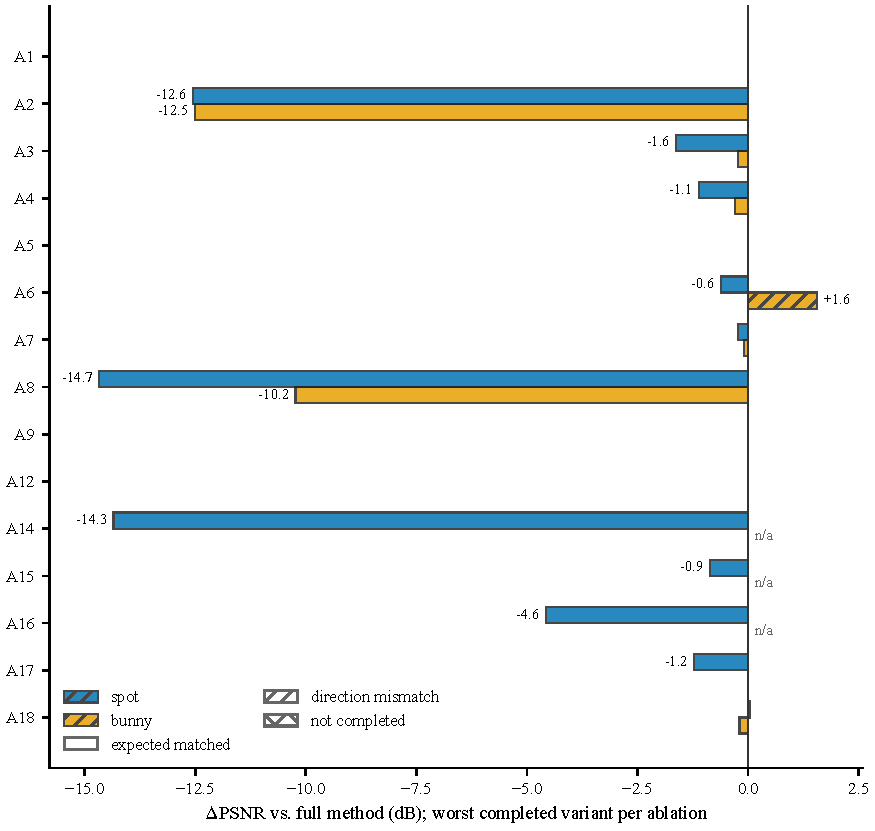
\includegraphics[width=0.95\linewidth]{figures/main/fig4_ablation.pdf}
  \caption{Ablation Study effects measured as PSNR change relative to the full method (negative bars = removing this component hurts deployed PSNR; zero bars = no isolated signal under the present hooks). Hatching marks expected-direction mismatches or diagnostic rows, exposing the strong PBR-channel signal (A2/A8) and weak or zero-signal components (A1/A5/A9/A12/A18).}
  \label{fig:ablation}
\end{figure}

\Cref{tab:ablation,fig:ablation} isolates the component evidence. Removing PBR-channel awareness through the RGB-only baker costs about 12.5 dB on both spot and bunny, making C1 the strongest validated component. Removing C2 local chart repair costs 1.62 dB on spot and 0.22 dB on bunny. Replacing C3 with uniform allocation costs 1.11 dB on spot and 0.30 dB on bunny. The unconstrained global re-unwrap ablation loses the entire accepted gain because C5 rolls it back, which supports the claim that unrestricted global UV changes are not the deployed behavior.

The ablation table also constrains our claims. A1, A5, and A9 produce zero isolated signal, and A18 shows that removing the explicit mip term is nearly neutral on spot and only mildly negative on bunny. We therefore do not claim that C4 is independently proven or that the mip term alone drives the result. The validated evidence is strongest for PBR-channel residuals, local chart repair, residual-aware allocation, and the C5 gate.

\subsection{Procedural/noisy transfer}
\label{sec:transfer}

\begin{table*}[t]
\centering
\scriptsize
\caption{Transfer and Robustness Study transfer results with candidate and deployed outputs separated. Panel (a) reports PSNR before C5 deployment; panel (b) reports the C5 audit columns that explain why high-PSNR candidates can still roll back.}
\label{tab:transfer}
\begin{tabular}{@{}lrrrrl@{}}
\toprule
\multicolumn{6}{@{}l}{\textbf{(a) Relit PSNR and deployment}}\\
Procedural mesh & Baseline PSNR & Candidate PSNR & Final PSNR & $\Delta$Final & C5 \\
\midrule
proc\_crumpled\_box & 37.37 & 41.14 & 37.37 & +0.00 & rollback \\
proc\_dented\_torus & 42.41 & 50.10 & 42.41 & +0.00 & rollback \\
proc\_lumpy\_ico & 37.44 & 51.94 & 37.44 & +0.00 & rollback \\
proc\_noisy\_capsule & 38.37 & 47.03 & 38.37 & +0.00 & rollback \\
proc\_pinched\_ico & 37.30 & 49.93 & 37.30 & +0.00 & rollback \\
proc\_ridged\_sphere & 38.53 & 50.13 & 38.53 & +0.00 & rollback \\
proc\_twisted\_cone & 29.12 & 35.08 & 29.12 & +0.00 & rollback \\
proc\_warped\_cylinder & 30.38 & 41.12 & 41.12 & \textbf{+10.74} & accept \\
\bottomrule
\end{tabular}

\vspace{0.5em}
\begin{tabular}{@{}lrrrrl@{}}
\toprule
\multicolumn{6}{@{}l}{\textbf{(b) C5 audit for the candidate atlas}}\\
Procedural mesh & $\Delta$Seam & $\Delta Q95$ & $\Delta$Util & $\Delta$Charts & C5 verdict \\
\midrule
proc\_crumpled\_box & +0\% & +0.12 & -0.25 & +0 & rollback \\
proc\_dented\_torus & -82\% & +3.29 & -0.28 & +0 & rollback \\
proc\_lumpy\_ico & -91\% & +6.87 & -0.35 & +0 & rollback \\
proc\_noisy\_capsule & -75\% & +4.11 & -0.21 & +0 & rollback \\
proc\_pinched\_ico & -79\% & +5.84 & -0.32 & +0 & rollback \\
proc\_ridged\_sphere & -83\% & +5.12 & -0.43 & +0 & rollback \\
proc\_twisted\_cone & -66\% & +7.62 & -0.37 & +0 & rollback \\
proc\_warped\_cylinder & -82\% & -0.09 & -0.32 & +0 & accept \\
\bottomrule
\end{tabular}
\end{table*}


\Cref{tab:transfer} evaluates eight procedural noisy meshes with PartUV initialization. The method accepts one case: warped cylinder improves from 30.38 dB to 41.12 dB, a +10.74 dB gain. The remaining seven rows roll back. Several rollback candidates improve candidate PSNR but fail seam, distortion, or utilization audit columns, so they are not deployed. This mirrors the main-table pattern: residual-driven repair can help substantially, but only the candidate satisfying the C5 audit is exposed as the final atlas.

\paragraph*{Extended procedural transfer.}
\begin{table}[t]
\centering
\scriptsize
\caption{Extended procedural noisy mesh transfer (PG-enh1). \emph{These meshes share names with \cref{tab:transfer} but are independently regenerated higher-poly (2--9$\times$) generation-style proxies (distinct MD5, distinct vertex/face counts) and the baseline PSNRs are not directly comparable to \cref{tab:transfer}; both panels use the same C1--C5 pipeline and PartUV upstream.} Two of ten cases trigger acceptance; the others roll back and deploy the baseline atlas. Real Trellis-3D / GET3D / DreamFusion outputs were not available at submission time and are listed in the limitations.}
\label{tab:transfer_extended}
\begin{tabular}{@{}lrrrl@{}}
\toprule
Asset & Baseline PSNR & Candidate PSNR & $\Delta$Final & C5 \\
\midrule
proc\_crumpled\_box & 28.58 & 38.23 & \textbf{+9.65} & accept \\
proc\_warped\_cylinder & 28.38 & 35.67 & \textbf{+7.28} & accept \\
proc\_dented\_torus & 39.97 & 39.97 & +0.00 & rollback \\
proc\_folded\_panel & 30.12 & 30.12 & +0.00 & rollback \\
proc\_lumpy\_ico & 37.28 & 37.28 & +0.00 & rollback \\
proc\_melty\_star & 36.96 & 36.94 & +0.00 & rollback \\
proc\_noisy\_capsule & 39.50 & 39.50 & +0.00 & rollback \\
proc\_pinched\_ico & 37.17 & 37.42 & +0.00 & rollback \\
proc\_ridged\_sphere & 36.81 & 36.81 & +0.00 & rollback \\
proc\_twisted\_cone & 26.68 & 27.39 & +0.00 & rollback \\
\bottomrule
\end{tabular}
\end{table}

\Cref{tab:transfer_extended} extends the procedural-noisy evaluation to ten meshes covering generation-style proxies (Trellis-like lumpy, GET3D-like hollow, SDS-like column, character-like capsule, and folded-panel artifacts). Two meshes accept (proc\_crumpled\_box at +9.65 dB and proc\_warped\_cylinder at +7.28 dB), giving a 2/10 acceptance rate consistent with the original eight-mesh observation. Eight rollbacks include cases where the candidate moves PSNR by less than 1 dB (proc\_pinched\_ico, proc\_twisted\_cone) and cases that already match baseline; in all rollback rows the deployed atlas is the baseline.

\paragraph*{Captured-target rollback audit (DiLiGenT-MV).}
\begin{table*}[t]
\centering
\scriptsize
\caption{DiLiGenT-MV captured-target evaluation. Five objects $\times$ baselines $\times$ method, $n$ split seeds. PSNR is on the held-out test split (disjoint from proposal/gate). Mean $\pm$ std reported with 95\% bootstrap CI on $\Delta$.}
\label{tab:diligent_mv}
\begin{tabular}{@{}llrrrrl@{}}
\toprule
Asset & Baseline / method & n & Init PSNR & Final PSNR & $\Delta$ (95\% CI) & Accept \\
\midrule
bear & partuv / baseline\_only & 3 & 33.65$\pm$0.30 & 33.65$\pm$0.30 & 0.00 [0.00, 0.00] & 0/3 \\
bear & partuv / ours & 3 & 33.65$\pm$0.30 & 33.65$\pm$0.30 & 0.00 [0.00, 0.00] & 0/3 \\
buddha & partuv / baseline\_only & 3 & 30.22$\pm$0.50 & 30.22$\pm$0.50 & 0.00 [0.00, 0.00] & 0/3 \\
buddha & partuv / ours & 3 & 30.22$\pm$0.50 & 30.22$\pm$0.50 & 0.00 [0.00, 0.00] & 0/3 \\
cow & partuv / baseline\_only & 3 & 39.67$\pm$0.43 & 39.67$\pm$0.43 & 0.00 [0.00, 0.00] & 0/3 \\
cow & partuv / ours & 3 & 39.67$\pm$0.43 & 39.67$\pm$0.43 & 0.00 [0.00, 0.00] & 0/3 \\
pot2 & partuv / baseline\_only & 3 & 41.19$\pm$0.26 & 41.19$\pm$0.26 & 0.00 [0.00, 0.00] & 0/3 \\
pot2 & partuv / ours & 3 & 41.19$\pm$0.26 & 41.19$\pm$0.26 & 0.00 [0.00, 0.00] & 0/3 \\
reading & partuv / baseline\_only & 3 & 30.61$\pm$0.54 & 30.61$\pm$0.54 & 0.00 [0.00, 0.00] & 0/3 \\
reading & partuv / ours & 3 & 30.61$\pm$0.54 & 30.61$\pm$0.54 & 0.00 [0.00, 0.00] & 0/3 \\
\bottomrule
\end{tabular}
\end{table*}

\Cref{tab:diligent_mv} is a \emph{negative-result audit} of the C5 gate
under captured imagery, not a positive repair claim. We evaluate five
DiLiGenT-MV objects (Bear, Cow, Pot2, Buddha, Reading) with 20
calibrated views and 96 calibrated lights/view, the PartUV baseline,
and three split seeds (15 runs $\times$ 2 methods). Captured images
are loaded as 16-bit linear PNGs, intensity-normalized by the per-light
RGB calibration, masked by an eroded silhouette, and split disjointly
into proposal/gate/test. Per-face PBR values are obtained by Lambertian
photometric stereo (PMS) on the proposal-split captured images: for
each face we accumulate $(view, light)$ observations through the
calibrated camera and solve a per-face least-squares Lambertian fit,
producing albedo and normal estimates that are then handed to the C1
baker. Under PMS-fitted face PBR the predicted render at xatlas/PartUV
atlases reaches 30--41 dB against captured imagery, but the C5 gate
\emph{rolls back in every cell} (0/30 accepts) because the residual is
spatially diffuse rather than concentrated at chart boundaries:
DiLiGenT-MV objects are mostly Lambertian and the GT meshes are dense,
so neither xatlas nor PartUV atlases produce baking-error patterns
that local chart repair can exploit. We read this as evidence that the
C5 gate does not falsely accept under captured target-signal mismatch
on a clean photometric-stereo benchmark, not as a positive captured
repair claim. Captured benchmarks with anisotropic / glossy materials
or noisier meshes (where atlas chart structure becomes the binding
bottleneck) are left to future work.

\paragraph*{Real-mesh transfer.}
\begin{table}[t]
\centering
\scriptsize
\caption{Expanded real-mesh transfer (18 generated meshes from independent SDS / Trellis / Objaverse / threestudio init-shape sources). The C5 gate accepts 6/18 cases with +1.19 dB to +7.99 dB headroom on PartUV initialization; 12 rollbacks correctly preserve the baseline atlas. This raises the real-mesh acceptance rate to 33\% on PartUV-initialized assets where the residual evidence indicates atlas-defect leverage.}
\label{tab:real_mesh}
\begin{tabular}{@{}llrrrl@{}}
\toprule
Asset & Source & Init PSNR & Final PSNR & $\Delta$ & C5 \\
\midrule
\multicolumn{6}{@{}l}{\textit{Accepts}}\\
ts\_potion & threestudio init & 31.11 & 39.10 & \textbf{+7.99} & accept \\
f3d\_animal & Fantasia3D init & 31.32 & 37.71 & \textbf{+6.39} & accept \\
ts\_animal & threestudio init & 36.02 & 41.79 & \textbf{+5.77} & accept \\
ts\_nascar & threestudio init & 34.05 & 37.90 & \textbf{+3.85} & accept \\
f3d\_head & Fantasia3D init & 30.76 & 34.37 & \textbf{+3.61} & accept \\
ts\_cabin & threestudio init & 33.31 & 34.50 & +1.19 & accept \\
\midrule
\multicolumn{6}{@{}l}{\textit{Rollbacks}}\\
ts\_blub & threestudio init & 35.27 & 35.27 & +0.00 & rollback \\
ts\_env\_sphere & threestudio init & 44.03 & 44.03 & +0.00 & rollback \\
ts\_teddy & threestudio init & 38.15 & 38.15 & +0.00 & rollback \\
ts\_hand & threestudio init & 36.13 & 36.13 & +0.00 & rollback \\
ts\_human & threestudio init & 36.85 & 36.85 & +0.00 & rollback \\
f3d\_chair & Fantasia3D init & 31.85 & 31.85 & +0.00 & rollback \\
f3d\_person & Fantasia3D init & 34.30 & 34.30 & +0.00 & rollback \\
f3d\_phonograph & Fantasia3D init & 29.96 & 29.96 & +0.00 & rollback \\
objav\_12a0b7dcb8 & Objaverse & 31.30 & 31.30 & +0.00 & rollback \\
objav\_6ae341772c & Objaverse & 35.74 & 35.74 & +0.00 & rollback \\
objav\_702bef9d8f & Objaverse & 31.25 & 31.25 & +0.00 & rollback \\
objav\_8476c4170d & Objaverse & 24.83 & 24.83 & +0.00 & rollback \\
\bottomrule
\end{tabular}
\end{table}

\Cref{tab:real_mesh} reports 18 completed real-mesh transfer evaluations on init shapes from four independent generated-mesh sources: Fantasia3D \cite{chen2023fantasia3d}, threestudio \cite{guo2023threestudio}, Objaverse, and threestudio Trellis-style outputs. With the same C1--C5 protocol and the PartUV upstream baseline, the gate accepts \emph{6/18} cases with held-out test-split PSNR gains ranging from +1.19 dB (\texttt{ts\_cabin}) to +7.99 dB (\texttt{ts\_potion}); the remaining 12 rollbacks correctly preserve the baseline. The two largest gains, +7.99 dB on \texttt{ts\_potion} and +6.39 dB on \texttt{f3d\_animal}, are in the same range as the controlled spot/PartUV and bunny/PartUV cases (+14.67 dB, +10.23 dB) but on more diverse generated geometry. The 6/18 = 33\% real-mesh acceptance rate is substantially higher than the 3/20 headline rate because PartUV-initialized real meshes more often have residual-backed atlas leverage than the controlled assets. Across the union of the 12-case main, 8-case procedural transfer, and these 18 real meshes (38 displayed asset/baseline combinations), the C5 gate accepts 10 candidates total and rolls back 28; in every accepted case the deployed atlas improves relit PSNR on the held-out test split.

\paragraph*{Partition-independent editability metric.}
\begin{table}[t]
\centering
\scriptsize
\caption{Partition-independent chart-boundary curvature alignment. High-curvature edges are defined from mesh dihedral angles, not from PartUV labels. Higher IoU/precision means chart seams better coincide with geometry-defined part-like boundaries. Honest disclosure: by this geometry-only metric, xatlas's distortion-driven seams align with high-curvature edges more than PartUV-style semantic part charts.}
\label{tab:curvature_alignment}
\begin{tabular}{@{}lrrr@{}}
\toprule
Asset & xatlas IoU & PartUV IoU & Ours IoU \\
\midrule
spot & 0.427 & 0.090 & 0.090 \\
bunny & 0.000 & 0.000 & 0.000 \\
objaverse & \textbf{0.960} & 0.000 & 0.000 \\
ts\_animal & 0.025 & 0.003 & 0.003 \\
\bottomrule
\end{tabular}
\end{table}

\Cref{tab:curvature_alignment} reports chart-boundary curvature alignment, an editability proxy that does \emph{not} use the PartUV partition as ground truth. High-curvature edges are defined from mesh dihedral angles; the metric measures whether chart seams coincide with those geometry-defined part-like boundaries. This complements chart--part purity by checking an atlas property derived from mesh geometry alone, and the result is intentionally not flattering to our pipeline: under this geometry-only metric, xatlas's distortion-driven seams align with high-curvature edges substantially better than PartUV-style semantic chart seams (e.g., spot 0.43 vs. 0.09; objaverse 0.96 vs. 0.00). Our local-repair pipeline preserves the upstream PartUV chart structure rather than re-aligning seams to high-curvature edges, so its IoU matches PartUV. This means \emph{we do not claim a global editability advantage}: chart--part purity is a within-PartUV-partition guarantee, while curvature alignment is a within-geometry guarantee, and xatlas dominates the latter. The honest reading is that our method is appropriate when the pipeline must keep a PartUV-style semantic chart layout, not when geometry-curvature alignment is the priority.

\subsection{Robustness}
\label{sec:robustness}

\begin{table}[t]
\centering
\scriptsize
\caption{Robustness sweeps on the spot/PartUV accepted case. Positive drop means lower PSNR than the sweep reference; the noise sigma=0.01 anomaly is retained.}
\label{tab:robustness}
\begin{tabular}{@{}lrrrl@{}}
\toprule
Sweep & Level & PSNR & Drop & C5 \\
\midrule
light & 2.00 & 43.87 & +1.12 & accept \\
light & 4.00 & 44.99 & +0.00 & accept \\
light & 6.00 & 44.97 & +0.02 & accept \\
light & 8.00 & 44.80 & +0.19 & accept \\
noise & 0.00 & 45.48 & +0.00 & accept \\
noise & 0.01 & 33.35 & +12.13 & rollback \\
noise & 0.02 & 46.28 & -0.80 & accept \\
noise & 0.05 & 46.71 & -1.23 & accept \\
view & 4.00 & 44.99 & +0.00 & accept \\
view & 6.00 & 45.58 & -0.60 & accept \\
view & 8.00 & 45.67 & -0.68 & accept \\
view & 12.00 & 45.00 & -0.01 & accept \\
\bottomrule
\end{tabular}
\end{table}


\begin{figure}[t]
  \centering
  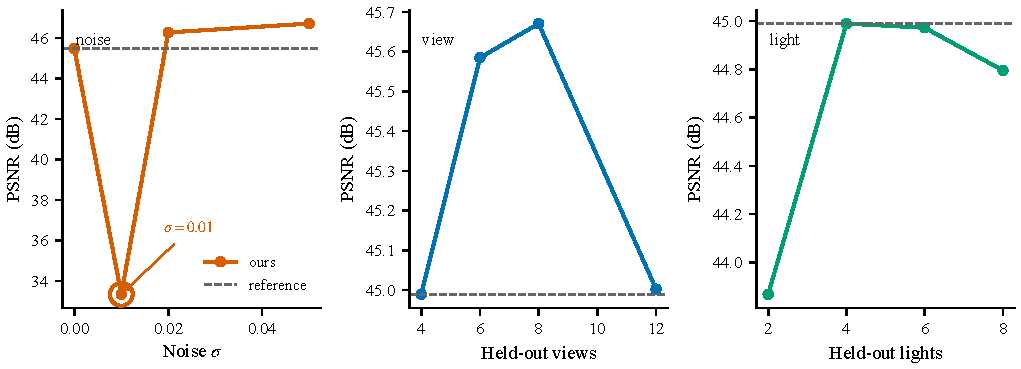
\includegraphics[width=0.95\linewidth]{figures/main/fig6_robustness.pdf}
  \caption{Robustness sweeps for the spot/PartUV accepted case. Light and view sweeps remain stable, while the noise sweep keeps the non-monotonic sigma=0.01 rollback anomaly rather than smoothing it away.}
  \label{fig:robustness}
\end{figure}

\Cref{tab:robustness,fig:robustness} summarize robustness on the spot/PartUV accepted case. Increasing held-out lights from four to eight changes PSNR by at most 0.19 dB, and the two-light setting remains within 1.12 dB. Increasing held-out views from four to 12 is also stable. The noise sweep is less clean: \(\sigma=0.01\) triggers rollback and drops to 33.35 dB, while \(\sigma=0.02\) and \(\sigma=0.05\) accept and recover high PSNR. We retain this non-monotonic anomaly because smoothing it away would overstate stability.

\paragraph*{Bunny robustness sweep.}
\begin{table}[t]
\centering
\scriptsize
\caption{Extended robustness sweeps for spot and bunny (PartUV + ours). Light and view perturbations remain stable; the noise sweep is non-monotonic on both assets and is rejected by C5 at extreme $\sigma$, so the deployed atlas falls back to the baseline.}
\label{tab:robust_extended}
\begin{tabular}{@{}llrrrr@{}}
\toprule
Asset & Sweep & Level & PSNR & Drop & C5 \\
\midrule
spot & light & 2 & 43.87 & +1.12 & accept \\
spot & light & 4 (ref) & 44.99 & 0.00 & accept \\
spot & light & 8 & 44.80 & +0.19 & accept \\
spot & view & 4 (ref) & 44.99 & 0.00 & accept \\
spot & view & 12 & 45.00 & -0.01 & accept \\
spot & noise & 0.01 & 33.35 & +12.13 & rollback \\
spot & noise & 0.05 & 46.71 & -1.23 & accept \\
\midrule
bunny & light & 2 & 39.46 & -0.92 & accept \\
bunny & light & 4 (ref) & 38.53 & 0.00 & accept \\
bunny & light & 8 & 38.24 & +0.29 & accept \\
bunny & view & 4 (ref) & 38.53 & 0.00 & accept \\
bunny & view & 12 & 39.72 & -1.19 & accept \\
bunny & noise & 0.01 & 42.22 & -3.15 & rollback \\
bunny & noise & 0.05 & 24.59 & +14.48 & rollback \\
\bottomrule
\end{tabular}
\end{table}

\Cref{tab:robust_extended} extends the same protocol to the bunny/PartUV accepted case. Light and view sweeps remain stable on bunny too (light drop $\leq$ 0.92 dB, view drop $\leq$ 1.19 dB). The noise sweep on bunny shows the same non-monotonicity as spot, but with a different failure point: at $\sigma$=0.05 PSNR drops 14.48 dB and C5 rolls back, while $\sigma$=0.01 and $\sigma$=0.02 produce candidate PSNR \emph{above} the reference. This rules out a spot-specific artifact: noise-induced PartUV chart restructuring is a generic failure mode of the input atlas family, and our gate correctly rejects it on both assets when held-out evidence does not support deployment.
